\typeout{Bewegingsherkenning met een smartphone}

\documentclass{article}
\usepackage[dutch]{babel}
\usepackage{ijcai11}
\usepackage{times}
\usepackage{graphicx}
\usepackage{pgfplots}
\usepackage{rotating}
\usepackage{tikz}
\usetikzlibrary{fit,arrows,calc,positioning,backgrounds}
\usetikzlibrary{patterns}


\tikzset{every fit/.append style=text badly centered}
\tikzset{class/.style={
      draw,
      rectangle,
      rounded corners=7pt,
      inner ysep=5pt,
    }
}

% voor deze packages: sudo apt-get install texlive-science
\usepackage[Algoritme]{algorithm}
\usepackage{algpseudocode}

\usepackage{subcaption}
%\usepackage{latexsym}  %optional

\title{Bewegingsherkenning met een smartphone}
\author{Arne De Brabandere\\
	arne.debrabandere@student.kuleuven.be
    \And
    Menno Keustermans\\
    menno.keustermans@student.kuleuven.be}
    
\tikzset{
    vertex/.style = {
        circle,
        fill            = black,
        outer sep = 2pt,
        inner sep = 1pt,
    }
}

\begin{document}

\maketitle

\begin{abstract}

Het herkennen van menselijke bewegingen is een belangrijk onderdeel van `context aware computing'. Uit de metingen van de accelerometer en gyroscoop van een smartphone kan de activiteit van de gebruiker bepaald worden. In het eerste deel van ons onderzoek zoeken we naar modellen om afzonderlijke activiteiten te herkennen. Het nauwkeurigste model wordt gevonden met de classificatiemethode Random Forests met een accuraatheid van 93\%. Vervolgens gebruiken we dit model om een sequentie van verschillende bewegingen te evalueren. We ontwikkelen hiervoor een algoritme dat de sequentie in opeenvolgende tijdsvensters van x aantal seconden knipt, die ook met een bepaald percentage kunnen overlappen. Uit experimenten blijkt dat hiervoor een tijdsvenstergrootte van vier tot zes seconden met een overlapping van 75\% het nauwkeurigst is met 84\% accuraatheid.

\end{abstract}

\section{Introductie}

Door de versnellingen en rotaties van menselijke bewegingen te meten, is het mogelijk om automatisch te herkennen welke activiteiten uitgevoerd worden. We maken hier een onderscheid tussen metingen van afzonderlijke activiteiten (\'e\'en activiteit per meting) en sequenties van activiteiten (verschillende activiteiten na elkaar in een meting). We gaan voor beide soorten metingen op zoek naar een methode om de activiteiten te herkennen.

Het nauwkeurig detecteren van menselijke bewegingen is een belangrijke doelstelling van `context aware computing'. Hierbij wordt software gekoppeld aan de gebruiker, zodat die bewust is van de omgeving en toestand van de gebruiker. Toepassingen hiervan bevinden zich bijvoorbeeld in e-gezondheid applicaties. Voor dit onderzoek werd gebruik gemaakt van een smartphone als bewegingssensor. Dit levert verschillende voordelen op. Het zijn namelijk populaire apparaten de dag van vandaag, die bovendien bruikbare ingebouwde sensoren (accelerometer en gyroscoop) hebben.

In deze paper wordt een oplossing gezocht voor twee probleemstellingen: (1) Welke classificatiemethode levert het nauwkeurigst model op om afzonderlijke activiteiten te herkennen? (2) Kunnen we dit model gebruiken om sequenties van verschillende activiteiten nauwkeurig te voorspellen?

De eerste probleemstelling wordt besproken in sectie 2. De oplossing verloopt in drie stappen (zie figuur 1 voor een overzicht). In de eerste stap worden gegevens verzameld (sectie 2.1). Vervolgens worden uit de gegevens features berekend (sectie 2.2). Die gebruiken we ten slotte om modellen te leren met behulp van classificatiemethodes (sectie 2.3).

Om een oplossing te vinden voor de tweede probleemstelling wordt het beste model van het eerste deel van het onderzoek gebruikt. De stappen van het proces om sequenties van activiteiten te herkennen verloopt in gelijkaardige stappen als die van het proces voor afzonderlijke activiteiten (zie figuur 5 voor een overzicht). Ten eerste moeten opnieuw gegevens verzameld worden (sectie 3.1). Vervolgens worden deze gegevens verwerkt (sectie 3.2). Om tenslotte de activiteiten van de sequenties te voorspellen, wordt gebruik gemaakt van een algoritme met drie parameters (sectie 3.3).

\subsubsection{Gerelateerd werk}

Zoals eerder vermeld, is bewegingsherkenning een belangrijk concept in 'context aware computing'. Hierdoor is er al veel onderzoek naar gedaan.

Zo werd er in de paper~\cite{Ravi and others:act.recogn.} van Ravi, Dandekar, Mysore en Littman onderzocht naar herkenning van afzonderlijke activiteiten met behulp van gegevens opgemeten door een externe accelerometer. Zij maakten gebruik van meta-level classifiers om modellen te genereren.

Ook andere papers~\cite{6dmotion} maken gebruik van externe accelerometers, maar zij verschillen dan in het gebruik van classifiers. Zo hebben Chen, Alregib en Juang onderzocht naar het gebruik van HMMs classifiers.

In ons onderzoek worden gegevens opgemeten waarbij de meetapparatuur zich bevindt rondom de bekken. Casale, Pujol en Radeva deden gegevens opmetingen met een accelerometer rondom de borstzone en vonden een nauwkeurig model met behulp van Random Forests.~\cite{act.rec.}

De meeste van deze genoemde papers hebben zich gefocust op het herkennen van afzonderlijke activiteiten. Deze paper focust zich naast de afzonderlijke activiteiten, ook op het herkennen van sequenties van activiteiten.



% bij 2 secties telkens "data collectie" + "data verwerking" + leermethodes + experimenten  +resultaten + conclusie

\section{Afzondelijke activiteiten}
\label{afzonderlijk}

%bron: http://tex.stackexchange.com/questions/46007/tikz-node-placement-and-arrow-drawing
\tikzstyle{d} = [rectangle, draw, fill=blue!20, node distance=0.5cm, text width=5em, text centered, minimum height=4em, thick]
\tikzstyle{o} = [rectangle, draw, fill=orange!20, node distance=0.5cm, text width=6em, text centered, rounded corners, minimum height=4em, thick]
\tikzstyle{l} = [draw, -latex',thick]
\begin{figure*}
\begin{center}
\begin{tikzpicture}[auto]

    % nodes

    \node [d] (activiteit) {Activiteit};
    
    \node [o, right=of activiteit, label={[xshift=0cm, yshift=0.1cm]MotionTracker}] (motiontracker) {Accelerometer\\Gyroscoop};
    
    \node [d, right=of motiontracker] (ruw) {Tijdstip\\Versnelling\\Rotatie};
    
    \node [o, right=of ruw, label={[xshift=0cm, yshift=0.1cm]MotionFingerprint}] (motionfp) {Features\\berekenen};
    
    \node [d, right=of motionfp] (instanties) {Instanties};
    
    \node [o, right=of instanties, label={[xshift=0cm, yshift=0.1cm]Weka}] (classificatie) {Classificatie-\\methodes};
    
    \node [d, right=of classificatie] (model) {Model};
    
    % paden
    
    \path [l] (activiteit) -- (motiontracker);
    \path [l] (motiontracker) -- (ruw);
    \path [l] (ruw) -- (motionfp);
    \path [l] (motionfp) -- (instanties);
    \path [l] (instanties) -- (classificatie);
    \path [l] (classificatie) -- (model);
\end{tikzpicture}
\end{center}
\caption{Proces voor zoeken van een model om afzonderlijke activiteiten te herkennen}
\label{fig:proces:afzonderlijk}
\end{figure*}

Het eerste probleem is om van een gegeven reeks samples van de accelerometer en gyroscoop van een smartphone de activiteit van een persoon te bepalen. Elke sample bestaat uit een reeks opeenvolgende tijdstippen met bijhorende x-,y-,z-versnellingen en rotatiesnelheden die werden opgemeten. We veronderstellen hier dat telkens \'e\'en afzonderlijke activiteit gemeten wordt.

We willen tien verschillende activiteiten kunnen herkennen:
\begin{itemize}
\item wandelen,
\item lopen,
\item fietsen,
\item een trap opwandelen,
\item een trap afwandelen,
\item springen,
\item niets doen (zitten, liggen, staan),
\item een lift versnelt omhoog,
\item een lift versnelt omlaag,
\item tanden poetsen.
\end{itemize}

In bovenstaande lijst hebben we tanden poetsen als moeilijke activiteit toegevoegd. De beweging lijkt sterk op niets doen en zal waarschijnlijk minder goed te herkennen zijn. De x-,y-,z-versnellingen van de verschillende activiteiten worden weergeven in figuur 8 (zie bijlage).

Merk op dat we in plaats van de activiteiten `lift naar boven of beneden nemen' enkel de versnelling van een lift naar boven of beneden in de lijst opnemen. Een lift naar boven nemen bevat dus de volgende activiteiten: lift versnelt omhoog~--~niets doen~--~lift versnelt omlaag. Het feit dat deze activiteiten ook `niets doen' bevatten, is de verklaring waarom we alleen de versnelling van een lift herkennen.
\\~\\
Het proces om de afzonderlijke activiteiten te herkennen verloopt in drie stappen. De eerste stap bestaat uit het verzamelen van de gegevens (zie figuur~\ref{fig:proces:afzonderlijk}). Hiervoor meten we de versnellingen en rotaties van de verschillende activiteiten. Als tweede stap worden features berekend uit de verzamelde gegevens. Deze zijn nodig om in de laatste stap modellen te leren met behulp van classificatiemethodes. Als criterium om de verschillende modellen te vergelijken, gebruiken we de accuraatheid als percentage van het aantal juiste geclassificeerde samples ten op zichte van het totaal aantal metingen met behulp van cross-validatie.

%TODO ook motivatie (waarom classificatiemethodes)

\subsection{Gegevensverzameling}

Alle gegevens werden opgemeten door de MotionTracker tool~\cite{meert and schietgat:motiontracker}. %TODO verwijzing met voetnoot: geschreven door ...
Dit is een Android-applicatie die de versnelling en rotatie (respectievelijk gemeten door de accelerometer en gyroscoop van de smartphone) meet aan 50Hz.  Als uitvoer geeft de applicatie een logbestand met de gemeten versnellingen (in de x-as, y-as en z-as; de z-as is evenwijdig met de gravitatie) en rotaties (in quaternion notatie) met bijhorende timestamps.

Voor elke meting werd de applicatie gestart alvorens de smartphone in de broekzak gestopt werd en gestopt na het uithalen. Daarom bevat het begin en einde van elke meting enkele seconden die niet tot de gemeten activiteit horen. Om het fout labelen te vermijden, werd na elke meting een stuk van de start en het einde van het logbestand weggeknipt, zodat elke meting exact \'e\'en activiteit bevat van vier tot twintig seconden lang. 

Op deze manier hebben we voor elke activiteit 22 metingen verzameld, opgemeten door twee verschillende personen. Om voldoende variatie te hebben, gebeurden de metingen op verschillende dagen. Ook hebben we ervoor gezorgd dat we niet telkens dezelfde broek droegen, aangezien de gemeten versnelling kan vari\"eren in verschillende broekzakken. Na elke meting werd het resulterende logbestand geknipt en gelabeld met de juiste activiteit.

%TODO figuur met verschillende activiteiten

\subsection{Gegevensverwerking: features berekenen}

Voor we classificatiemethodes kunnen gebruiken, moeten we eerst features berekenen. Dit zijn parameters die we uit de samples van de accelerometer en gyroscoop kunnen halen. Om de verschillende features te berekenen, maken we gebruik van de MotionFingerprint tool~\cite{meert and schietgat:motionfingerprint}. %TODO verwijzing naar tool 


%TODO uitleggen waarom we features berekenen

MotionFingerprint\footnote{MotionFingerPrint is te vinden op: http://dsip.cs.kuleuven.be/materials} berekent in totaal 134 features\footnote{Het aantal features is afhankelijk van de instellingen van de tool.} verdeeld onder vier soorten:
\begin{itemize}
\item \textit{Statistische features:} gemiddelde en standaardafwijking van z- en xy-versnelling en vermogen, correlatie tussen z- en xy-versnelling, etc. 
 
\item \textit{Fourier transformatie:} amplitudes horende bij bepaalde frequenties, pieken, etc.

\item \textit{Wavelet transformatie:} gemiddelde van de co\"effici\"enten per schaal, energie per schaal, etc.

\item \textit{Hidden Markov Models:} log-likelihood voor de verschillende HMM modellen. Voor elke activiteit wordt een model berekend uit zes metingen die apart werden gehouden. (Daarom worden ook in de rest van de paper slechts 16 van de 22 metingen gebruikt.)
\end{itemize}

%TODO uitleggen dat we verder voor de classificatiemethodes telkens 16 metingen gebruiken en dat we de andere 8 apart houden om HMM modellen te leren!

Na het berekenen van de features hebben we voor elke meting een set van parameters. Elke set vormt een instantie van de training set om een model te leren.

\subsubsection{Feature selectie}
%Waarom
Tussen de verschillende soorten features is er verschil in berekeningstijd en hoeveelheid informatie. Zo kunnen statistische features in het algemeen tegen een lagere kost berekend worden ten op zichte van Fourier transformatie features. In sommige toepassingen (zoals smartphone applicaties) kan het daarom interessant zijn om slechts een deel van het totaal aantal features te berekenen en juist diegene die de meeste informatie bevatten.

%Voorgestelde Oplossing
Met behulp van feature selectie onderzoeken we hoeveel features van het totaal aantal features van elke soort nodig zijn om een redelijke accuraatheid te behalen. Om de features met de meeste informatie te vinden, maken we gebruik van Weka's \emph{InfoGainAttributeEval} klasse\footnote{meer informatie over deze klasse is te vinden op: http://weka.sourceforge.net/doc.dev/weka/attributeSelection/
InfoGainAttributeEval.html}. %TODO voetnoot naar weka informatie gain
 Deze klasse evalueert de waarde van elke feature met behulp van information gain.

%Evaluatie
Om vervolgens de geselecteerde features te evalueren maken we gebruik van dubbele cross-validatie. Bij de eerste cross-validatie (10-fold) wordt de gegevensset telkens verdeeld in een training en test set. Voor elke training set selecteren we de beste features met het proces dat hierboven werd beschreven, gebruik makend van een tweede cross-validatie (2-fold). Met de geselecteerde features wordt een model opgesteld met behulp van de Random Forests classificatiemethode in Weka. Het gevonden model wordt uiteindelijk ge\"evalueerd op de test set van de eerste cross-validatie.
	
%Resultaten
In figuur~\ref{fig:1} worden de resulaten voor de verschillende soorten features getoond. We zien dat we met enkel de statistische features al een accuraatheid van 90\% behalen. Zelfs met de helft van de features kan het model al met een accuraatheid van 80\% activiteit voorspellen. We stellen vast dat van het grote aantal Fourier tranformatie features slechts een tiental nodig zijn om een nauwkeurigheid van 80\% te bekomen. De features die hierbij geselecteerd worden zijn voornamelijk lagere frequenties ($<2.5$ Hz) volgens het xy-vlak. Wavelet transformatie features lijken minder goed te werken met slechts 70\% accuraatheid. Tenslotte merken we in de laatste grafiek op dat de Hidden Markov Models enkel degelijk werken wanneer alle features gebruikt worden.

\begin{figure}[htb]
\centering

  \begin{subfigure}[b]{.49\linewidth}
    \centering
    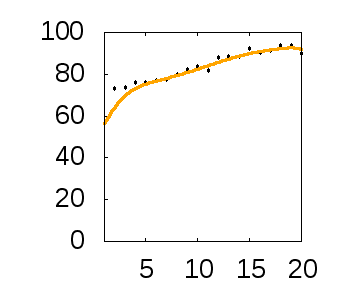
\includegraphics[width=0.99\textwidth]{figures/StatisticFeatures}
    \caption{Statistische features}\label{fig:1a}
  \end{subfigure}% 
  \begin{subfigure}[b]{.49\linewidth}
    \centering
    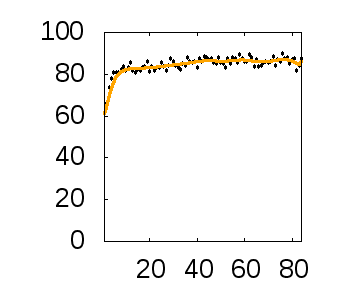
\includegraphics[width=.99\textwidth]{figures/FFTFeatures}
    \caption{FFT features}\label{fig:1b}
  \end{subfigure} \\
  \begin{subfigure}[b]{.49\linewidth}
    \centering
    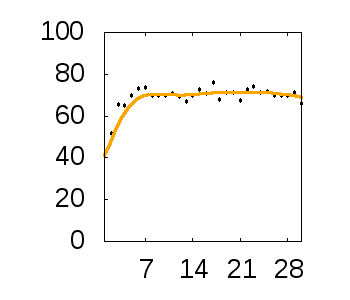
\includegraphics[width=.99\textwidth]{figures/DWTFeatures}
    \caption{Wavelet features}\label{fig:1c}
  \end{subfigure}
  \begin{subfigure}[b]{.49\linewidth}
    \centering
    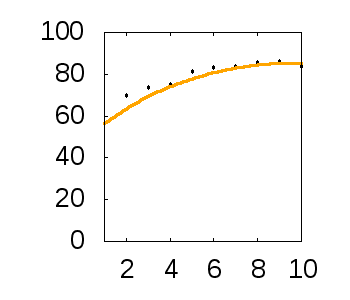
\includegraphics[width=.99\textwidth]{figures/HMMFeatures}
    \caption{HMM features}\label{fig:1e}
  \end{subfigure} \\
  

  \caption{Resultaten van het feature selectie experiment: op de x-as wordt steeds het aantal features van elke soort features geplot en op de y-as de accuraatheid (in percentages) van het model dat door Random Forests geleerd werd.}\label{fig:1}
\end{figure}

Voor de rest van het onderzoek wordt gebruik gemaakt van de volledige set features.



\subsection{Classificatiemethodes}

We gebruiken classificatiemethodes om een model te zoeken om afzonderlijke activiteiten te herkennen. We vergelijken enkele veel voorkomende methodes: beslissingsbomen, Random Forests, k-Nearest Neighbours, Naive Bayes en Support Vector Machines. De methodes leren telkens een model uit de instanties met de hierboven beschreven features voor de verschillende activiteiten. Hieronder wordt kort de werking van de vernoemde methodes beschreven:

\begin{itemize}
\item \textit{Beslissingsbomen} zijn bomen waarvan de interne knopen features voorstellen en de bladknopen \'e\'en (of meerdere) labels bevatten. Een tak in de boom stelt een test voor op de feature van de knoop waaruit de tak vertrekt. Om een nieuwe instantie te classificeren worden de juiste takken gevolgd tot in een bepaalde bladknoop. De instantie wordt dan geclassificeerd als het label in die bladknoop.
\item \textit{Random Forests} zijn combinaties van beslissingsbomen met een willekeurig deel van de trainingset en een willekeurig deel van de features. Bij de classificatie van een nieuwe instantie `stemt' elke boom op een label. De instantie krijgt vervolgens het label met de meeste stemmen.
\item \textit{k-Nearest Neighbours} classificeert nieuwe instanties door te zoeken naar de k dichtstbijzijnde instanties in de trainingset. Dit zijn de instanties waarvan de waarden voor de features het dichtst bij die van de te classificeren instantie ligt. Hieruit wordt het meest voorkomende label gekozen.
\item \textit{Naive Bayes} is een probabilistische classifier die gebruik maakt van voorwaardelijke kansen. De features van een te classificeren instantie worden hier als een vector $\mathbf{F} = (F_1, ..., F_n)$ voorgesteld. Een label $C_1$ is waarschijnlijker dan een label $C_2$ wanneer $P(\mathbf{F}|C_1) P(C_1) > P(\mathbf{F}|C_2) P(C_2)$. Hierin kunnen de kansen $P(\mathbf{F}|C_i)$ en $P(C_i)$ voor alle labels $C_i$ uit de trainingset berekend worden. Bij het classificeren wordt het meest waarschijnlijke label gekozen.
\item \textit{Support Vector Machines} beschouwt de features als een multidimensionele ruimte. De instanties zijn dan punten in de featureruimte. Bij het leren worden de instanties lineair van elkaar gescheiden een hypervlak, zodat de instanties aan de ene kant van het vlak een ander label hebben dan die aan de andere kant. Wanneer de instanties niet lineair te scheiden zijn, worden ze getransformeerd met een \textit{kernel functie}. We gebruiken hier LibSVM, %TODO bron
waarbij binaire (\'e\'en-tegen-\'e\'en) classificatie gedaan wordt: elk hypervlak scheidt de instanties van 2 verschillende labels. Een nieuwe instantie wordt geclassificeerd door elke binaire classificatie als een stem voor een label te beschouwen. Het label met het grootste aantal stemmen wordt gekozen.
\end{itemize}

\subsection{Experimenten en resultaten}
\label{afzonderlijk:experimenten}

Om de methodes te evalueren, maken we gebruik van de Weka Machine Learning Toolkit~\cite{waikato:weka}. %TODO bronvermelding
Die bevat classifiers die de hierboven vermelde methodes implementeren. Voor beslissingsbomen maken we gebruik van de J48 classifier, een implementatie van het C4.5 algoritme. %TODO bronvermelding
Verder gebruiken we IBk voor k-Nearest Neighbours en LibSVM voor Support Vector Machines.

De evaluatie gebeurt met 10-fold cross-validatie. Hierbij worden de instanties op tien verschillende manieren opgesplitst zodat telkens 90\% van de instanties als trainingset wordt gebruikt om een model uit te leren. Op de overige 10\% wordt het model ge\"evalueerd. De accuraatheid van elke methode wordt dan berekend als het gemiddelde percentage van correct geclassificeerde instanties in de verschillende testsets.

In figuur \ref{fig:methodes}
wordt de accuraatheid van de verschillende classificatiemethodes vergeleken. We zien dat Random Forest de hoogste accuraatheid (93,75\%) geeft voor de metingen. Ook J48 geeft een goede accuraatheid (87.5\%). De hogere accuraatheid van Random Forest ten opzichte van beslissingsbomen is te verklaren door het feit dat Random Forest minder kans op overfitting heeft.~\cite{breiman:randomforests} Naive Bayes lijkt ook goed te werken, terwijl met IBk en vooral LibSVM een lagere accuraatheid bereikt wordt. De accuraatheid van de methodes kan echter wel verbeterd worden door de parameters de optimaliseren.

\begin{figure}[h]
\centering
\begin{tikzpicture}
\begin{axis}[
    ybar,
    xtick=data,
    ymin=0,
    xticklabels from table={Data/methodes.dat}{methode},
    xticklabel style={align=center},
    nodes near coords,
    ylabel={Accuraatheid (\%)}
]

\addplot table [
    x=xpos,
    y=accuraatheid
] {Data/methodes.dat};

\end{axis}
\end{tikzpicture}
\caption{Accuraatheid van classificatiemethodes}
\label{fig:methodes}
\end{figure}

\begin{figure*}
\begin{center}
{ \footnotesize
\begin{tabular}{ c | c | c | c | c | c | c | c | c | c | l }
     \begin{sideways} Wandelen       \end{sideways}
  &  \begin{sideways} Lopen          \end{sideways} 
  &  \begin{sideways} Fietsen        \end{sideways} 
  &  \begin{sideways} Trap op        \end{sideways} 
  &  \begin{sideways} Trap af        \end{sideways} 
  &  \begin{sideways} Springen       \end{sideways} 
  &  \begin{sideways} Niets doen     \end{sideways} 
  &  \begin{sideways} Lift omhoog    \end{sideways} 
  &  \begin{sideways} Lift omlaag    \end{sideways} 
  &  \begin{sideways} Tanden poetsen \end{sideways} 
  &  $\leftarrow$ \parbox[b]{1.8cm}{geclassificeerd\\als} \\   \hline
 16 &    &    &    &    &    &    &    &    &    & Wandelen           \\   \hline
    & 16 &    &    &    &    &    &    &    &    & Lopen              \\   \hline
    &    & 16 &    &    &    &    &    &    &    & Fietsen            \\   \hline
    &    &    & 15 &  1 &    &    &    &    &    & Trap op            \\   \hline
    &    &    &    & 16 &    &    &    &    &    & Trap af            \\   \hline
    &    &    &    &    & 16 &    &    &    &    & Springen           \\   \hline
    &    &    &    &    &    & 14 &    &    &  2 & Niets doen         \\   \hline
    &    &    &    &    &    &    & 10 &  6 &    & Lift omhoog        \\   \hline
    &    &    &    &    &    &    &  1 & 15 &    & Lift omlaag        \\   \hline
    &    &    &    &    &    &    &    &    & 16 & Tanden poetsen
\end{tabular}
}
\end{center}
\caption{Confusion matrix voor Random Forest}
\label{fig:confusionmatrix}
\end{figure*}

Voor het model dat door Random Forest geleerd werd, hebben we in figuur \ref{fig:confusionmatrix} een confusion-matrix geplot. Het valt op dat activiteiten met grote versnellingen -- wandelen, lopen, fietsen en springen -- goed te herkennen zijn. Alle metingen voor deze activiteiten worden immers correct geclassificeerd door het model. Niets doen, lift versnelt omhoog/omlaag en tanden poetsen hebben kleinere versnellingen dan de andere activiteiten. We zien dat twee metingen van niets doen als tanden poetsen worden geclassificeerd. Ook lift omhoog en omlaag worden gemakkelijk met elkaar verward. Omwille van de kleine versnellingen zijn de verschillen tussen de activiteiten subtieler, wat een verklaring kan zijn waarom deze activiteiten moeilijker te herkennen zijn.
\\~\\
%korte conclusie
We kunnen voor de afzonderlijke activiteiten besluiten dat door Random Forests het nauwkeurigste (93,75\%) model geleerd wordt.


\section{Sequenties van activiteiten}

\tikzstyle{d} = [rectangle, draw, fill=blue!20, node distance=0.5cm, text width=6em, text centered, minimum height=4em, thick]
\begin{figure}
\begin{center}
\begin{tikzpicture}

    % nodes

    \node [d] (sequentie) {Sequentie};
    
    \node [o, right=of sequentie] (motiontracker) {Accelerometer\\Gyroscoop};
    
    \node [d, right=of motiontracker] (ruw) {Tijdstip\\Versnelling\\Rotatie};
    
    \node [d, below=4em of sequentie] (vensters) {Tijds-\\vensters};
    \node [o, right=of vensters] (afzonderlijk) {Algoritme 2:\\activiteiten\\herkennen};
    \node [d, right=1.8em of afzonderlijk] (voorspelling) {Predicties};
    
    \begin{pgfonlayer}{background}
    		\node [class, inner xsep=0.6em, fit=(sequentie) (motiontracker) (ruw)] (metingen) {};
        \node [class, inner xsep=0.6em, fit=(vensters) (afzonderlijk), label={[xshift=-1.6cm, yshift=0.1cm]Algoritme 1}] (algoritme) {};
    \end{pgfonlayer}
    
    % path
    
    \path [l] (sequentie) -- (motiontracker);
    \path [l] (motiontracker) -- (ruw);
    \path [l] (metingen) -- (algoritme);
    \path [l] (vensters) -- (afzonderlijk);
    \path [l] (afzonderlijk) -- (voorspelling);
    
\end{tikzpicture}
\end{center}
\caption{Proces om predicties te maken voor een sequentie van activiteiten}
\label{fig:proces:sequenties}
\end{figure}

Bij het herkennen van afzonderlijke activiteiten bevat elke meting exact \'e\'en activiteit. De classificatiemethodes die we hiervoor gebruiken zijn dus niet rechtstreeks toepasbaar op metingen waarin verschillende activiteiten na elkaar gebeuren. Daarom gaan we op zoek naar een methode om voor een sequentie van activiteiten te bepalen welke activiteiten daarin gedaan worden en wanneer.

In figuur~\ref{fig:proces:sequenties} wordt het proces beschreven om sequenties van activiteiten te herkennen. We beginnen met het opmeten van de versnelling en rotatie van verschillende sequenties. In het algoritme dat we zullen bespreken, worden de sequenties vervolgens in overlappende tijdsvensters geknipt. De activiteiten van de tijdsvensters worden bepaald met behulp van een model om afzonderlijke activiteiten te herkennen. Ten slotte worden hiermee predicties gemaakt voor de sequenties.

\subsection{Gegevensverzameling}
\label{seq:gegevens}

Met behulp van de MotionTracker~\cite{meert and schietgat:motiontracker} applicatie werd opnieuw de versnelling en rotatie gemeten, maar nu van meerdere activiteiten na elkaar. In totaal zijn vier sequenties van elk ongeveer drie minuten lang opgemeten: twee verschillende combinaties van activiteiten, telkens door twee personen opgemeten. De ene combinatie bevat de activiteiten wandelen, trap op en af, niets doen, lopen en springen. De andere bevat wandelen, trap op en af, niets doen en lift omhoog en omlaag. Omdat lift versnellingen moeilijk van elkaar te onderscheiden zijn door het model voor afzonderlijke activiteiten (zie sectie~\ref{afzonderlijk:experimenten}), verwachten we dat de tweede combinatie moeilijker te herkennen is dan de eerste.

Om de metingen te evalueren, werd elke sequentie gelabeld. Elke label bevat de start- en eindtijden van de verschillende activiteiten in de bijhorende meting. De delen die niet gelabeld werden, beschouwen we als ruis. Ruis defini\"eren we als niet-herkenbare activiteit. Het gaat om periodes met activiteiten die niet tot de tien activiteiten behoren die we kunnen herkennen. De smartphone in de broekzak stoppen is hier een voorbeeld van.

\subsection{Gegevensverwerking}

Aangezien de modellen voor afzonderlijke activiteiten niet rechtstreeks kunnen toegepast worden op sequenties, moeten de sequenties geknipt worden in delen die wel \'e\'en activiteit bevatten. We doen dit door de sequenties in tijdsvensters op te splitsen. De vensters hebben een lengte van enkele seconden en kunnen overlappen opdat er meer kans is dat een venster \'e\'en activiteit bevat. We defini\"eren een overlapping als het percentage van de lengte van een tijdsvenster dat ook tot het eerst volgende tijdsvenster hoort. In figuur \ref{fig:overlap} wordt ge\"illustreerd wat een overlapping van bijvoorbeeld 75\% betekent.

\begin{figure}[h]

\begin{subfigure}[b]{.90\linewidth}
\centering
\begin{tikzpicture}[width=0.8\textwidth]
\draw [d] (-3.5,2) node (v1) {} rectangle (0,1);
\draw [o] (v1) rectangle (-6.5,1);
\node at (-6.5,0.8) {0};
\node at (-0.1,0.8) {12};
\node at (-4.4,0.8) {4};
\node at (-2.5,0.8) {8};
\end{tikzpicture}
\caption{Sequentie van twee activiteiten: De linkerbalk is activiteit 1 en de rechterbalk is activiteit 2}
\end{subfigure}\\

\begin{subfigure}[b]{.90\linewidth}
\begin{tikzpicture}[scale=0.8, transform shape]

\draw [o] (-6.5,0.5) rectangle (-3.5,0);
\draw [d] (-3.5,0.5) rectangle (-2.5,0) node (v3) {};
\draw [o] (-5.5,-0.8) rectangle (-3.5,-1.3) node (v2) {};
\draw [d] (v2) rectangle (-1.7,-0.8);\definecolor{}{HTML}{F0F0EF}\definecolor{}{HTML}{F0F0EF}

\draw [<->] (-5.5,-0.3) -- node[below] {75\%} (-2.5,-0.3);
\draw [dotted] (-5.5,0) -- (-5.5,-0.7);
\draw [dotted] (-2.5,0) -- (-2.5,-0.8);
\node at (-5.5,-1.5) {2};
\node at (-1.8,-1.5) {9};
\end{tikzpicture}
\caption{Tijdsvensters met een overlapping van 75\%}
\label{fig:overlap}
  \end{subfigure} \\

\begin{subfigure}[b]{.90\linewidth}
\centering
\begin{tikzpicture}[scale=0.8, transform shape]
\draw [o] (-7.5,-2) rectangle (-4.5,-2.5);
\draw [o] (-7.5,-3) rectangle (-5.5,-3.5);
\draw [d] (-3.5,-2) rectangle (-4.5,-2.5);
\draw [d] (-3.5,-3) rectangle (-5.5,-3.5);
\draw [o] (-2,-2) rectangle (-1.5,-2.5);
\draw [d] (-2,-3) rectangle (-1.5,-3.5) node (v4) {};
\draw [o] (-1,-2.5) rectangle (1.3,-3);
      % !TIKZEDT NOPREVIEW
    
\draw [decorate, decoration={brace, amplitude=5pt}](-1.4,-1.8) -- (-1.4,-3.6);
\node at (-2.8,-2.2) {= 60\%:};
\node at (-2.8,-3.2) {= 35\%:};
\node at (0.2,-2.3) {Voorspelling:};
\node at (-1,-3.2) {2};
\node at (1.2,-3.2) {2.5};
\end{tikzpicture}
\caption{Voorspelling maken: het eerste tijdsvenster beslist voor 60\% dat het de eerste activiteit bevat. Het tweede tijdsvenster besluit voor slechts 35\% dat hij de tweede activiteit bevat. Hierdoor besluit het algoritme dat voor tijstip 2s t.e.m. 2.5s activiteit 1 uitgevoerd wordt}

\end{subfigure}
  \caption{Voorstelling van het algoritme om sequenties van activiteiten te classificeren. In figuur (a) wordt een sequentie van twee activiteiten getoond over 12 seconden. Vervolgens worden er tijdsvensters met overlapping van 75\% geknipt in figuur (b). Tenslotte wordt een voorspelling gemaakt in figuur (c).}\label{fig:algoritme}

\end{figure}

\subsection{Algoritme}

Bij het voorspellen van de activiteiten van een sequentie maken we gebruik van de tijdsvensters. We beschrijven een algoritme waarmee voor elke halve seconde van een sequentie een voorspelling kan gemaakt worden voor de activiteit die daarin gebeurde. Een algemeen overzicht van het algoritme is te vinden in figuur 6.

Het algoritme heeft drie parameters nodig: de lengte van de tijdsvensters in seconden, de overlapping ervan als een percentage en een ruis cutoff kans. De laatste parameter wordt verder verduidelijkt. In sectie 3.4 worden experimenten uitgevoerd om de waarden voor deze parameters te kiezen zodat de voorspellingen van het algoritme zo correct mogelijk zijn.

Voor de pseudo-code van het algoritme verwijzen we naar Algoritme~\ref{alg:sequentie}. De eerste stap bestaat uit het splitsen van de sequentie in tijdsvensters met de gegeven lengte en overlapping. Vervolgens wordt voor elk deel van een halve seconde lang van de sequentie gecontroleerd welke tijdsvensters dat deel bevatten. Deze vensters zijn samen met de ruis cutoff kans de parameters van Algoritme~\ref{alg:deel} om de activiteit van het deel van de sequentie te bepalen. Hierbij wordt voor elk venster een voorspelling gemaakt met behulp van een model om afzonderlijke activiteiten te classificeren. In sectie~\ref{afzonderlijk} bleek Random Forests het best te werken. Daarom gebruiken we hier het model dat door deze methode geleerd werd. Voor elk venster laten we ook de kans berekenen dat het voorspelde label correct is. Bij Random Forests wordt deze kans bepaald als het percentage van de bomen die dat label voorspellen. %TODO klopt dit? want ik vind er niet onmiddellijk iets over...
Als minstens twee vensters met het deel van de sequentie overlappen, houdt het algoritme geen rekening met de kansen wanneer de voorspelde labels van de vensters gelijk zijn. In dat geval wordt als voorspelling het label van de tijdsvensters voorspeld. Anders controleert het algoritme of er een label is met een kans groter dan de ruis cutoff kans. Indien dat zo is, wordt voor het deel van de sequentie het label met de grootste kans als activiteit voorspeld. Wanneer alle kansen onder de ruis cutoff kans liggen, zal de voorspelling `Ruis' zijn.

\begin{algorithm}
  \caption{Activiteiten van een sequentie (met start en eind timestamp in seconden) voorspellen door als uitvoer een lijst terug te geven met voor elke halve seconde de voorspelde activiteit}
  \label{alg:sequentie}
  \begin{algorithmic}[0]
    \State \textbf{Parameters:}\\
    $lengte$ van de tijdsvensters (in seconden) \\
    $overlapping$ van de tijdsvensters (percentage) \\
    $cutoff$ voor ruis (kans) \\
    \State Splits de sequentie op in tijdsvensters met gegeven $lengte$ en $overlapping$ \\
    \For{$t$ = $start$; $t$ $\le$ $einde$; $t$ += $0.5s$}
      \State $vensters$ = tijdsvensters die $t$ en $t+0.5s$ bevatten
      \State $voorspellingen$[$t$] = \textsc{activiteit}($vensters,cutoff$) \\
      \Comment{zie Algoritme \ref{alg:deel}}
    \EndFor \\
    \State \textbf{return} $voorspellingen$
  \end{algorithmic}
\end{algorithm}

\begin{algorithm}
  \caption{Activiteit van een deel van een sequentie bepalen, met een gegeven lijst van tijdsvensters en een ruis cutoff kans}
  \label{alg:deel}
  \begin{algorithmic}[0]
    \Procedure{activiteit}{$vensters, cutoff$}
      \State $labels$ = voorspelde activiteiten voor $vensters$ 
      \State $kansen$ = kansen voor de $labels$ \\
      \Comment{berekend door model van Random Forests} \\
      \If{aantal $vensters$ $\ge$ 2 \textbf{and} alle $labels$ gelijk}
        \State \textbf{return} $labels$[$0$]
      \Else
        \If{$kansen$[$i$] $>$ $cutoff$ voor een $i$}
          \State \textbf{return} $labels$[$i$] met $kansen$[$i$] maximaal
        \Else
          \State \textbf{return} `Ruis'
        \EndIf
      \EndIf
    \EndProcedure
  \end{algorithmic}
\end{algorithm}

\subsection{Experimenten}
\label{experimenten}

We evalueren het algoritme door het toe te passen op de vier verschillende sequenties die we opgemeten hebben (zie sectie~\ref{seq:gegevens}). Op die manier gaan we op zoek naar optimale waarden voor de parameters. De parameters moeten zodanig gekozen worden dat de voorspellingen van het algoritme zo nauwkeurig mogelijk zijn. We verwachten dat de tijdsvensters vier seconden lang moeten zijn om lift omhoog en omlaag te kunnen herkennen, aangezien deze activiteiten ongeveer vier seconden duren. Wanneer we daarbij een overlappingspercentage van 75\% kiezen, zullen de tijdsvensters steeds 1s verschuiven. Op die manier zullen de tijdsvensters waarschijnlijk vaker \'e\'en activiteit bevatten. Verder verwachten we dat voor de ruis cutoff een kans van 50\% een redelijke waarde zal zijn. Zo worden voorspellingen steeds met minstens 50 \% zekerheid gemaakt. 

Om de accuraatheid van de voorspellingen van het algoritme te kunnen evalueren, defini\"eren we eerst hoe we die berekenen. Zoals eerder vermeld, werden de opgemeten sequenties gelabeld zodat gekend is wanneer de verschillende activiteiten in elke meting starten en eindigen. Voor delen die niet gelabeld werden, veronderstellen we dat die `Ruis' als label hebben. We zullen de voorspellingen van het algoritme vergelijken met deze labels. Dit doen we door per halve seconde van de sequentie te controleren of de voorspelling overeenkomt met het label. Deze controle wordt echter niet gedaan voor overgangen in de sequentie: dat zijn delen van de sequentie die op maximaal 1 seconde van een start- of eindtijd van een gelabelde activiteit liggen. De accuraatheid wordt dan berekend door van alle gecontroleerde voorspellingen het percentage correcte voorspellingen te bepalen.

\subsection{Resultaten}

In figuur~\ref{fig:3d} worden de verschillende combinaties van de tijdvenster- en overlappingsgrootte getoond met de behaalde accuraatheid. Indien we de x-as volgen (door de overlapping constant te houden), zien we dat naarmate de tijdsvenstergrootte stijgt, ook de accuuraatheid stijgt. Er wordt een maximum gehaald rond de vier tot zes seconden, daarna daalt de accuuraatheid terug. Bij het volgen van de y-as (met een constante tijdsvenstergrootte), constateren we dat hoe groter het overlappingspercentage wordt, hoe nauwkeurigere voorspellingen gemaakt kunnen worden.

%TODO 
\begin{figure}[h]
\centering
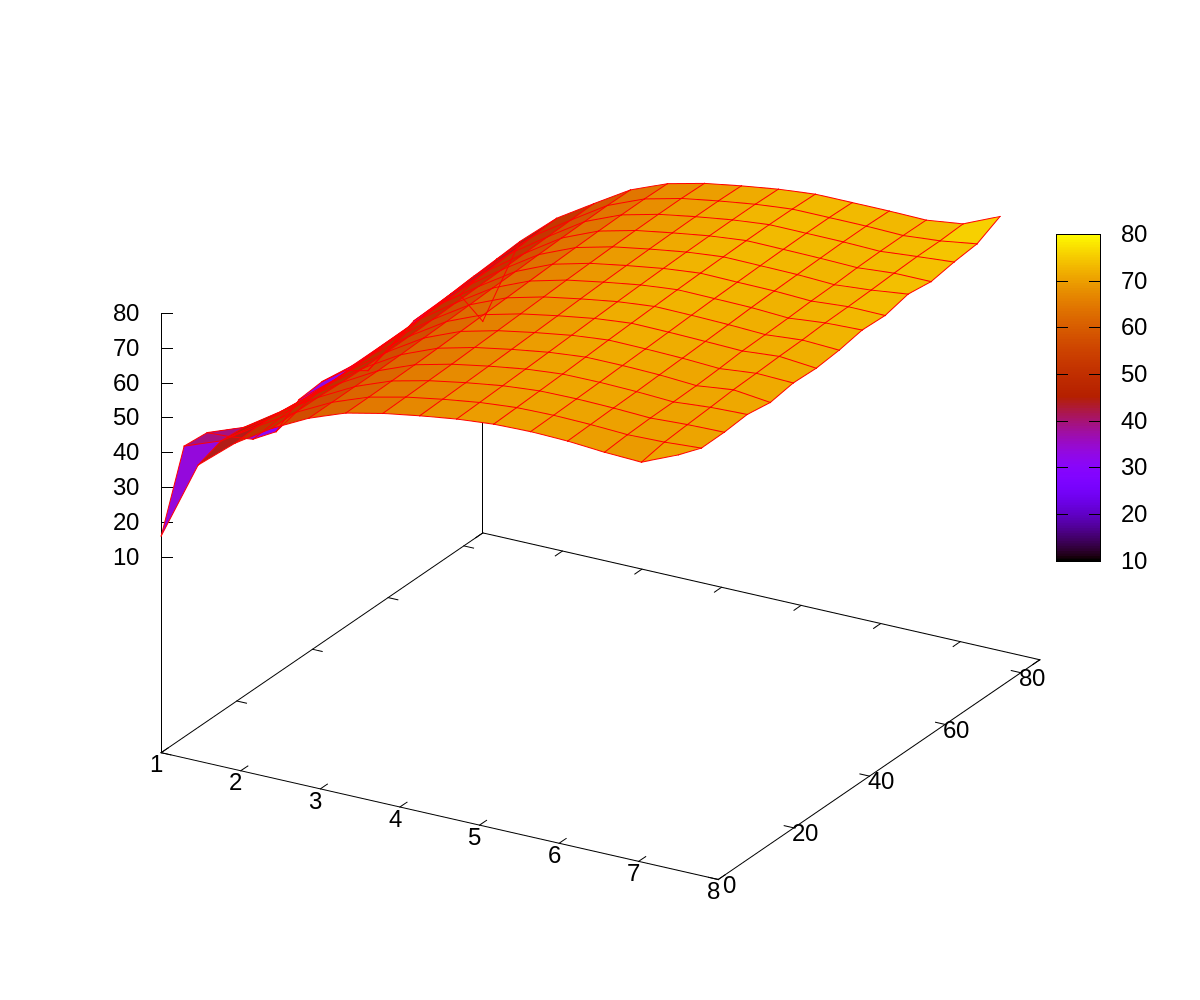
\includegraphics[width=0.5\textwidth]{figures/3dplot}
\caption{3D-plot dat de resultaten toont van het experiment (besproken in sectie 3.4). Op de x-as wordt de venstergrootte geplot in seconden. Op y-as zijn de overlappingen te zien in procenten. Uitvoering van het algoritme met de combinatie van deze parameters resulteert in een accuraatheid (geplot op de z-as)}
\label{fig:3d}
\end{figure}

Deze resultaten komen overeen met de hypothese die eerder gemaakt werd. De meeste activiteiten duren enkele seconden lang. Liftversnellingen bijvoorbeeld duren ongeveer vier seconden. Hierdoor is te verklaren waarom de tijdsvensters langer dan vier seconden moeten zijn. Tijdvensters van \'e\'en of twee seconden zijn niet altijd lang genoeg om een hele periode van een activiteit te bevatten. Grotere tijdsvensters leveren een lagere accuuraatheid op omdat de kans dat \'e\'enzelfde venster meerdere activiteiten bevat groter is. Daardoor is het moeilijker om de juiste activiteit te herkennen. De stijgende nauwkeurigheid voor toenemende overlappingsgrootte was ook te verwachten. Hoe groter de overlapping, hoe meer voorspellingen gemaakt kunnen worden per halve seconde van de sequentie. Hierbij moet wel een trade-off gemaakt worden: meer voorspellingen maken vraagt immers meer tijd.

Uit het vorige experiment kunnen we concluderen dat de optimale venstergrootte vier tot zes seconden is in combinatie met een overlappingspercentage van 75\%. Deze waarden samen met 50\% ruis cut-off leveren een gemiddelde nauwkeurigheid van 84\% voor de opgemeten sequenties.
\\~\\

%Korte conclusie
Voor de sequentie van activiteiten kunnen we concluderen dat voor ons algoritme de optimale venstergrootte vier tot zes seconden is in combinatie met 75\% overlapping. Er wordt een gemiddelde accuraatheid behaald van 84\%

	

\section{Conclusie}

Het doel van dit onderzoek was om een model te vinden om afzonderlijke bewegingen te herkennen. Vervolgens gebruikten we dit model om een sequentie van verschillende activiteiten te evalueren.

	In sectie 2 werden twee experimenten uitgevoerd in verband met afzonderlijke activiteiten. Het eerste experiment betreft de feature selectie. Hierbij werd onderzocht hoeveel features nodig zijn om een een voldoende nauwkeurig model te vinden. Het resultaat was dat enkel statistische features een model opleveren met 90\% nauwkeurigheid. We kunnen bij hetzelfde experiment ook concluderen dat van de 80 Fourier transformatie features slechts een tiental nodig zijn.
	In het tweede experiment werden verschillende classificatiemethodes met elkaar vergeleken. We maakten gebruik van vijf veel voorkomende machine learning technieken: beslissingsbomen, Random Forests, k-Nearest Neighbours, Naive Bayes en Support Vector Machines. Van deze methodes kwam Random Forests als beste naar boven met een nauwkeurigheid van 93,75\%.
	
	In sectie 3 werden sequenties van activiteiten ge\"evalueerd. Hiervoor hebben we een algoritme ontwikkeld waarvan de pseudocode besproken werd in sectie 3.3. 

Het algoritme vereist drie parameters: een tijdsvenstergrootte in seconden, een overlappingspercentage en een een ruis cutoff kans. Uit het experiment in sectie 3.4
bleek dat de optimale waarde voor de tijdsvenstergrootte vier tot zes seconden is en 75\% overlappingen een goede accuraatheid geven. De waarden werden getest op sequenties van ongeveer 3 minuten lang met steeds 4 \'a 5 verschillende activiteiten. Met behulp van het model van Random Forests (dit is het model dat gevonden werd in sectie 2.4
) werd er een gemiddelde nauwkeurigheid van 84\% gevonden.


%TODO voor afzonderlijke activiteiten EN (?) voor sequenties

\section{Verder werk}

Ondanks het feit dat tijdens dit onderzoek een redelijk model werd gevonden, kan dit altijd verder verbeterd worden.

\subsection{Afzonderlijke activiteiten}

Het model van de afzonderlijke activiteiten kan verbeterd worden door de gegevensverzameling te vergroten. Dit betekent dat meer gegevens verzameld moeten worden door meerdere proefpersonen. Hierdoor kan een algemener model berekend worden voor de verschillende afzonderlijke activiteiten, waardoor het model nauwkeurigere voorspellingen kan maken bij de sequenties van activiteiten.

Bovendien kunnen er modellen gegenereerd worden voor nieuwe activiteiten. Het toevoegen van extra activiteiten zal zoals eerder vermeld ook meer gegevens vragen.

\subsection{Sequenties van activiteiten}

Het algoritme voor sequenties van activiteiten te evalueren kan ook nog verder geoptimaliseerd worden. 
	Zo zijn bepaalde overgangen van activiteiten totaal onmogelijk. Het herkennen van fietsen na een liftversnelling is bijvoorbeeld onwaarschijnlijk. Zulke overgangen kunnen gefilterd worden door het gebruik van Markov ketens. Verder hebben we tijdens het onderzoek gemerkt dat soms enkele seconden als tanden poetsen herkend worden tijdens niets doen. Ook dit is onwaarschijnlijk en zou gefilterd kunnen worden met behulp van HMMs.

Tijdens het onderzoek werd geen rekening gehouden met de performantie (noch snelheid, noch geheugengebruik). Deze kan verder onderzocht en eventueel verbeterd worden.

	


Tenslotte is het nog mogelijk om het algoritme te implementeren in een smartphone-applicatie.

\section{Dankwoord}

Hierbij willen we graag Wannes Meert en Leander Schietgat bedanken. Eerst en vooral voor hun raad en ondersteuning. Ten tweede voor het ter beschikking stellen van de tools: MotionTracker en MotionFingerPrint.

%TODO bronvermelding!

%% The file named.bst is a bibliography style file for BibTeX 0.99c
\bibliographystyle{named}
\bibliography{paper}


\clearpage
\newpage

\section{Bijlage}
\begin{figure*}
\centering

  \begin{subfigure}[b]{.49\linewidth}
    \centering
    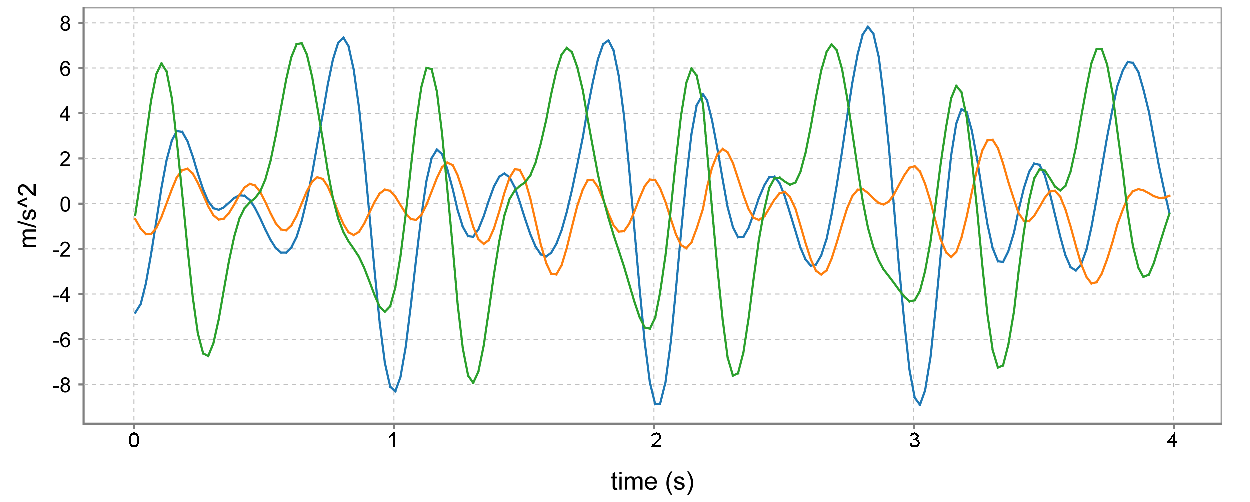
\includegraphics[width=0.99\textwidth]{figures/wandelen}
    \caption{Wandelen}\label{fig:1a}
  \end{subfigure}% 
  \begin{subfigure}[b]{.49\linewidth}
    \centering
    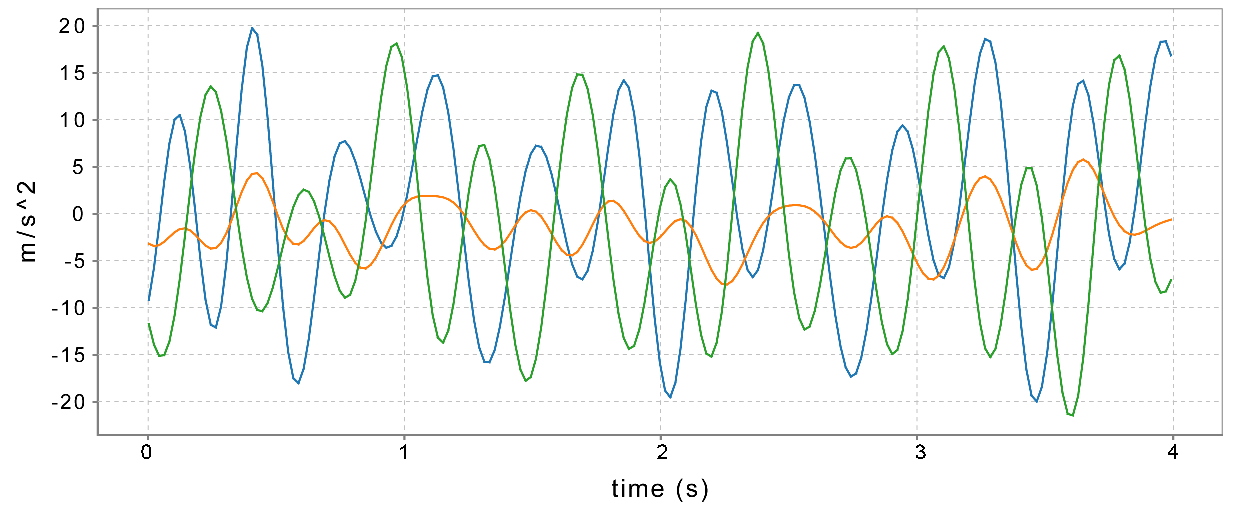
\includegraphics[width=.99\textwidth]{figures/lopen}
    \caption{Lopen}\label{fig:1b}
  \end{subfigure} \\~\\
  \begin{subfigure}[b]{.49\linewidth}
    \centering
    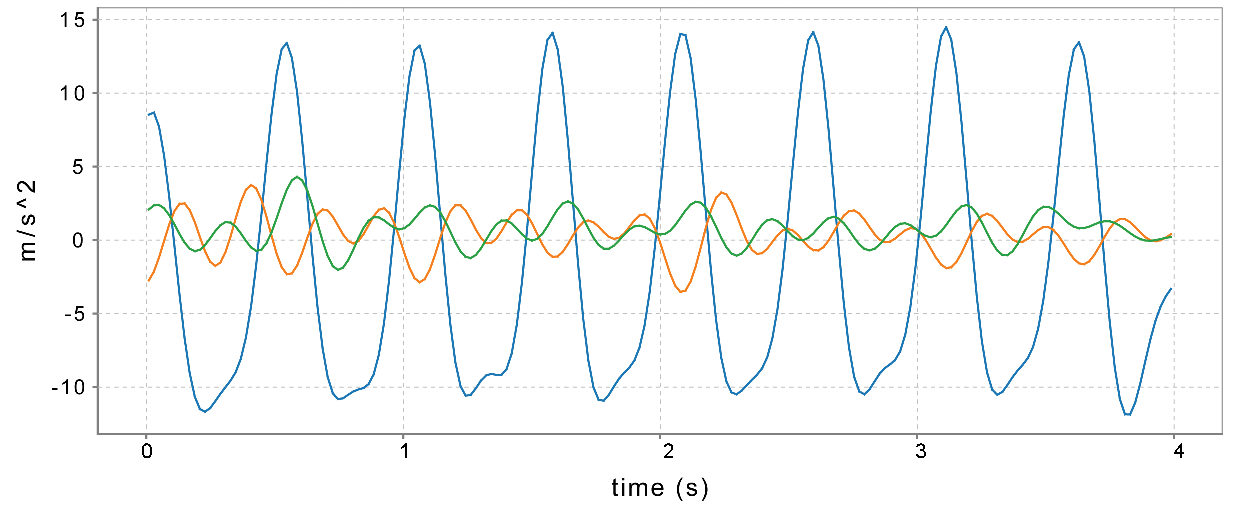
\includegraphics[width=.99\textwidth]{figures/springen}
    \caption{Springen}\label{fig:1c}
  \end{subfigure}
  \begin{subfigure}[b]{.49\linewidth}
    \centering
    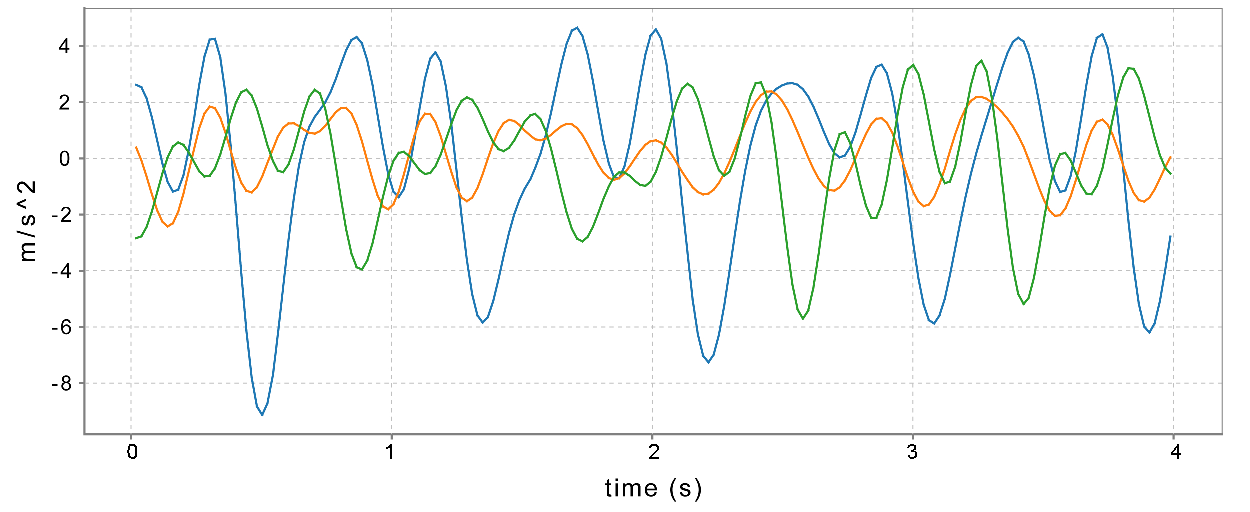
\includegraphics[width=.99\textwidth]{figures/fietsen}
    \caption{Fietsen}\label{fig:1d}
  \end{subfigure} \\~\\
  \begin{subfigure}[b]{.49\linewidth}
    \centering
    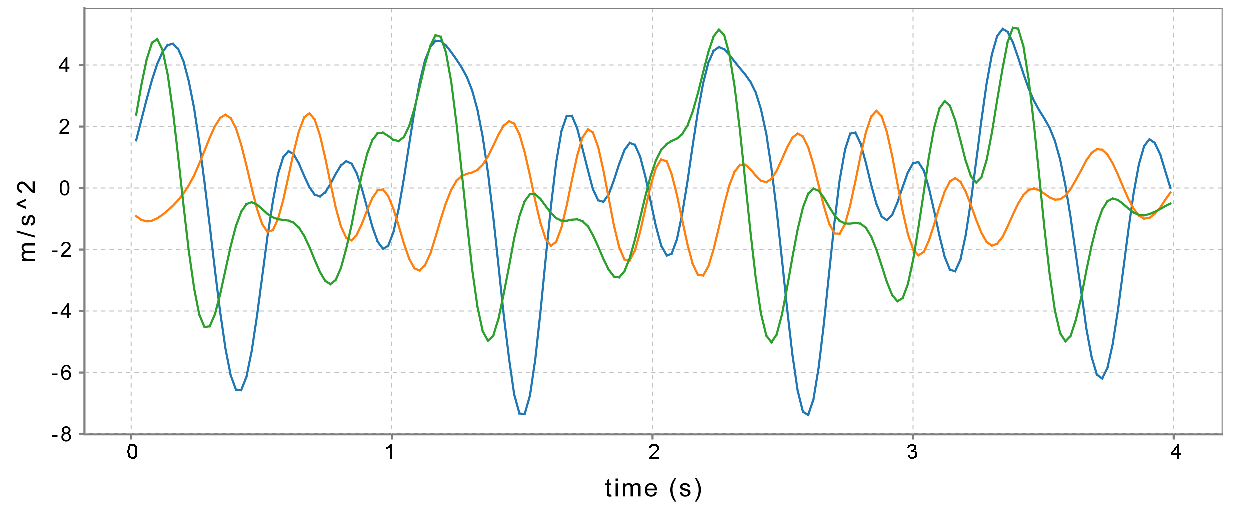
\includegraphics[width=.99\textwidth]{figures/trapop}
    \caption{Trap opwandelen}\label{fig:1e}
  \end{subfigure} 
  \begin{subfigure}[b]{.49\linewidth}
    \centering 
    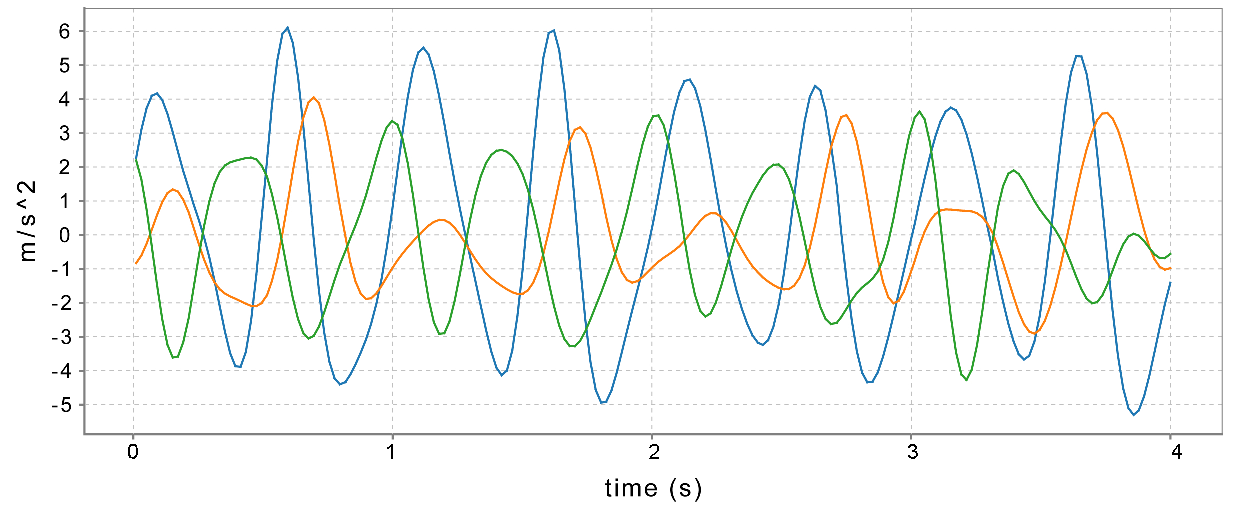
\includegraphics[width=.99\textwidth]{figures/trapaf}
    \caption{Trap afwandelen}\label{fig:1f}
  \end{subfigure} \\~\\
  \begin{subfigure}[b]{.49\linewidth}
    \centering
    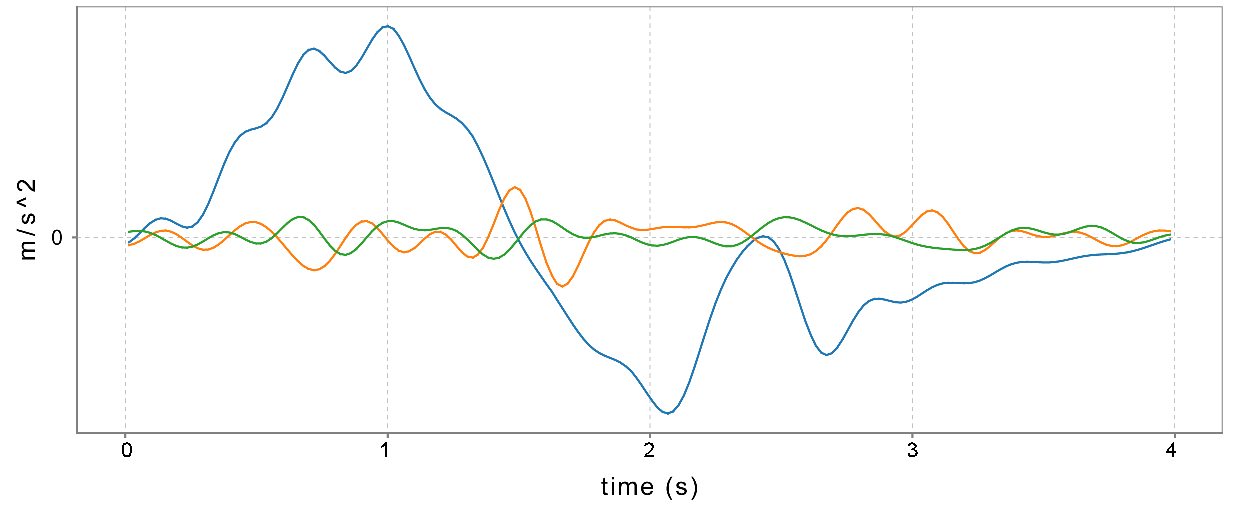
\includegraphics[width=.99\textwidth]{figures/liftau}
    \caption{Lift versnelt omhoog}\label{fig:1g}
  \end{subfigure}
  \begin{subfigure}[b]{.49\linewidth}
    \centering
    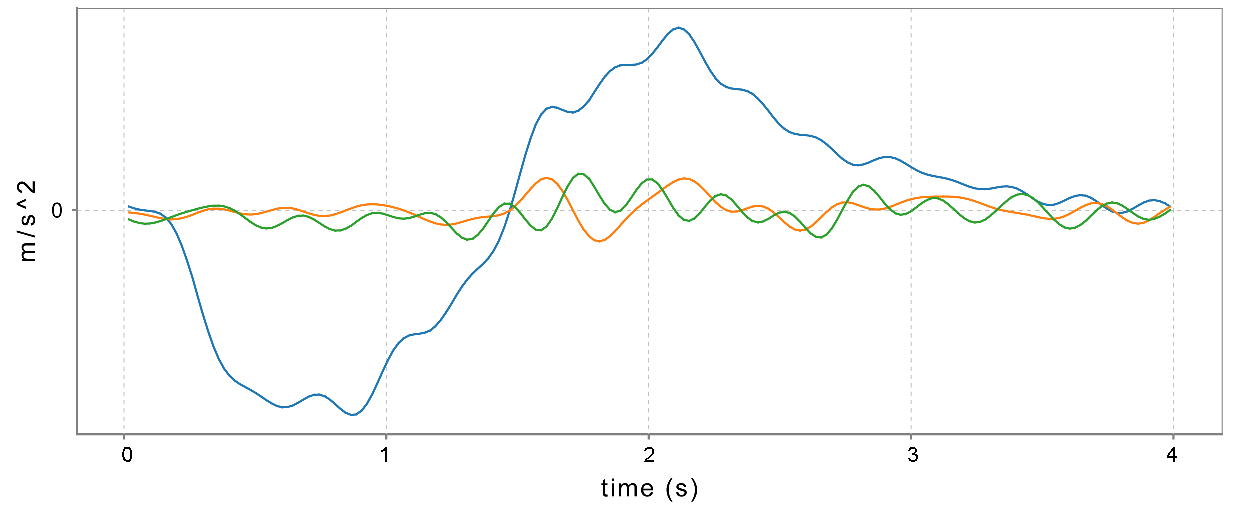
\includegraphics[width=.99\textwidth]{figures/liftad}
    \caption{Lift versnelt omlaag}\label{fig:1h}
  \end{subfigure} \\~\\
  \begin{subfigure}[b]{.49\linewidth}
    \centering
    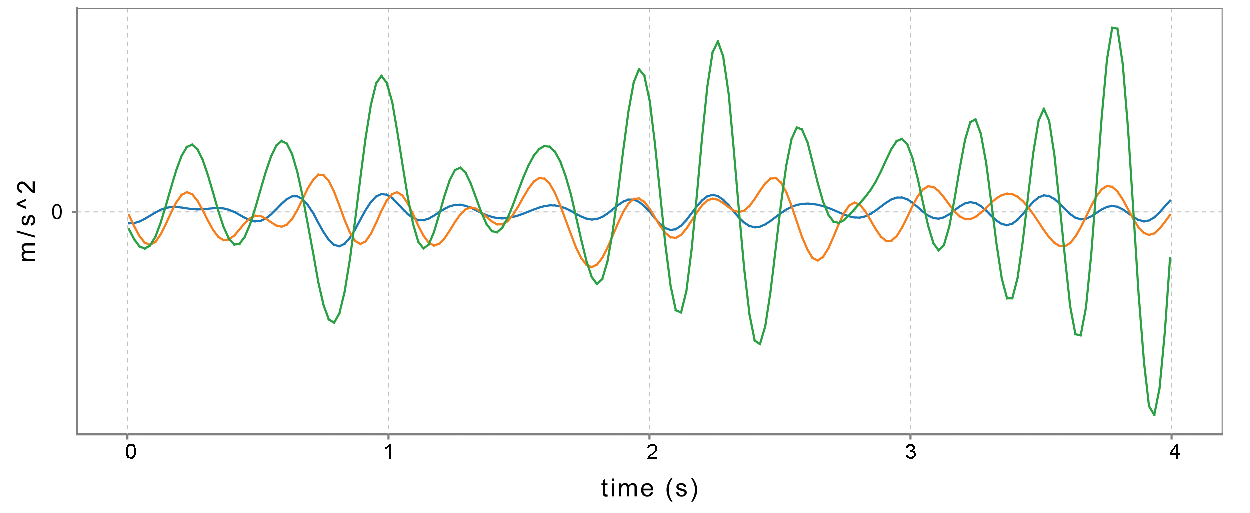
\includegraphics[width=.99\textwidth]{figures/tandenpoetsen}
    \caption{Tanden poetsen}\label{fig:1i}
  \end{subfigure}
  \begin{subfigure}[b]{.49\linewidth}
    \centering
    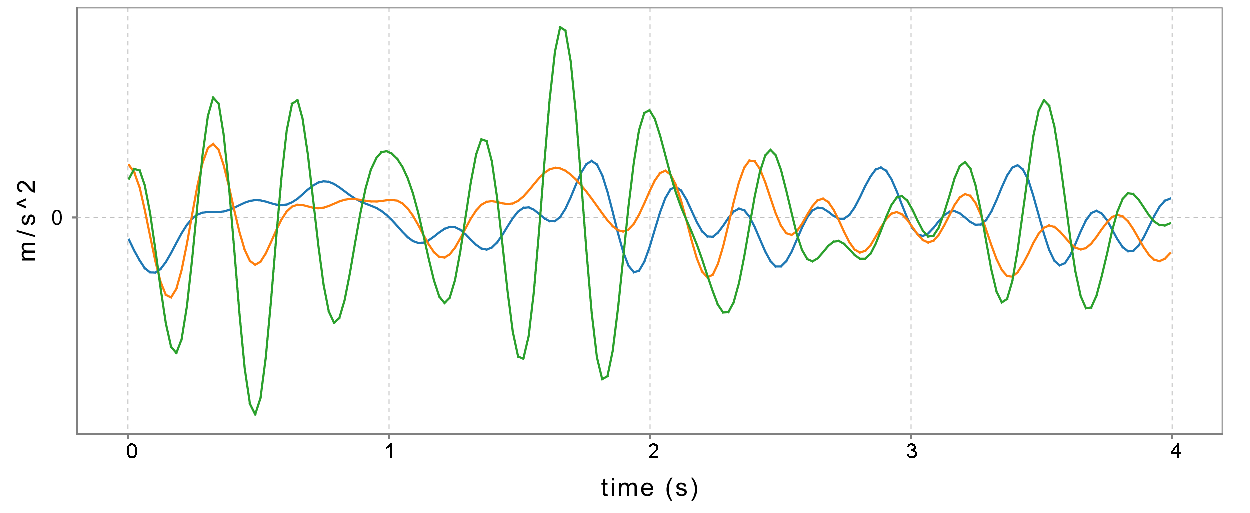
\includegraphics[width=.99\textwidth]{figures/nietsdoen}
    \caption{Niets doen}\label{fig:1j}
  \end{subfigure} \\
  \begin{subfigure}[b]{.49\linewidth}
    \centering
    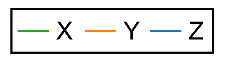
\includegraphics[width=.25\textwidth]{figures/legend}
  \end{subfigure}
  

  \caption{De tien verschillende activiteiten die afzonderlijk opgemeten werden voor dit onderzoek. Hierbij moet opgemerkt worden dat versnelling (y-as) niet op elke figuur dezelfde stap heeft }\label{fig:1}
\end{figure*}

\end{document}

